% ---------------------------------------------------------------------
% §7: Production Polyglot Stack
% ---------------------------------------------------------------------
\setcounter{section}{6}
\section{Production Polyglot Stack}
\label{sec:polyglot-stack}

The deterministic, sub-millisecond retrieval primitive formalized in
\S\ref{sec:formalization} is implemented in four production languages,
each contributing a distinct layer of the three-plane architecture
(\S\ref{sec:introduction}, §\ref{sec:clock-drift}). This section
documents the polyglot stack at the level of \emph{what language owns
which invariant}, deferring the line-by-line code excerpts to
Appendices~\ref{app:rust-dsvh}--\ref{app:telemetry}.

\subsection{Layer Partitioning: SRP / APG / ARL}

The three-plane architecture maps cleanly onto three language ecosystems.
We summarize the partition in Table~\ref{tab:polyglot-partition} and
discuss each row below.

\begin{table}[t]
\centering
\caption{Polyglot partition of the three-plane architecture. SRP =
Sub-Millisecond Retrieval Plane; APG = Asymmetric Prefill Gateway; ARL
= Agentic Reasoning Layer. The choice of language for each plane is
governed by the dominant invariant the plane must enforce, not by
team familiarity.}
\label{tab:polyglot-partition}
\vspace{2pt}
\begin{tabular}{@{}lllll@{}}
\toprule
Plane & Lang & Crate / Module & LOC & Invariant Enforced \\
\midrule
SRP & Rust & \texttt{dsvh} & 1{,}842 &
  Bitwise-deterministic projection, lock-free reads \\
APG & Go & \texttt{apg} & 2{,}108 &
  Stochastic eviction horizon, zero-prefill probes \\
ARL & Python & \texttt{rademacher\_embedder} & 412 &
  Reference reproduction, FTS5 corpus indexing \\
Bench & Rust & \texttt{ccebh} & 686 &
  Cache-locality-aware cold-cache benchmarks \\
\bottomrule
\end{tabular}
\end{table}

\paragraph{Sub-Millisecond Retrieval Plane (SRP).}
The SRP is the deterministic, lock-free plane that owns the FNV-1a
projection, the $L_2$ spherical normalization, and the cosine
similarity ranking. It is implemented in Rust because the dominant
invariant is \emph{bitwise determinism} under concurrent readers: every
corpus scan must produce the same byte sequence regardless of which
thread executes the scan, and the lock-free reads are guaranteed by
Rust's borrow checker plus the explicit \texttt{Arc<RwLock<Inner>>}
design documented in the operator-side audit and Appendix~\ref{app:rust-dsvh}. The Rust
implementation produces the $640$\,ns match latency ($\sigma = 85$\,ns)
reported in \S\ref{sec:benchmarks} and is the canonical reference for
all four formulas (FNV-1a, $L_2$, cosine, throughput).

\paragraph{Asymmetric Prefill Gateway (APG).}
The APG is the stochastic-control plane that owns the Eviction Horizon
$\mathcal{H}_{\text{evict}}$, the Weibull survival identification, and
the Zero-Prefill Keep-Alive Probes. It is implemented in Go because the
dominant invariant is \emph{concurrent goroutine isolation}: the APG
must run $K \ge 16$ concurrent probe goroutines on a single $1{,}000$-
document corpus without deadlock, race-condition, or probe-flood
contention. Go's goroutine scheduler plus the \texttt{context.Context}
cancellation primitives give us deterministic shutdown and bounded
resource usage under load. The Go implementation owns the
$\mathbf{1}_{\text{hit}}$ and $\mathbf{1}_{\text{miss}}$ indicator
collection that feeds the Bayesian posterior over the upstream TTL
state.

\paragraph{Agentic Reasoning Layer (ARL).}
The ARL is the autonomous-agent plane that owns the corpus ingestion,
the LLM chunking, and the FTS5 indexing. It is implemented in Python
because the dominant invariant is \emph{ecosystem breadth}: the ARL
must interface with the operator-side agent harness, the
\texttt{corpus indexer}, and the FTS5 SQLite
indexer, all of which are Python-first. The ARL is the only plane that
ships to end users as a \emph{reference reproducer}; the Rust and Go
planes are documented as pseudocode in Appendix~\ref{app:rust-dsvh} and
Appendix~\ref{app:apg-go} respectively.

\paragraph{Cold-Cache Edge Benchmark Harness (CCEBH).}
The CCEBH is the cache-locality-aware benchmarking plane that owns the
cold-cache reset, the $99$th-percentile tail latency measurement, and
the cross-substrate comparison. It is implemented in Rust because the
dominant invariant is \emph{cache-line granularity}: the CCEBH must
measure the impact of $L_1 / L_2 / L_3$ cache pressure on the
match-latency distribution, which requires pinning buffers to specific
NUMA nodes and forcing \texttt{clflush} via the
\texttt{cpuid\_clflush} intrinsic. The CCEBH owns the $25/25$
concurrency-stability result reported in \S\ref{sec:benchmarks}.

\subsection{Language-Specific Determinism Properties}

Each language in the polyglot stack has a different notion of
``deterministic''. We document the four that matter for the
mathematical correctness of the FNV-1a + $L_2$ + cosine + throughput
stack:

\begin{enumerate}
\item \textbf{Rust} guarantees bitwise determinism by default. The
\texttt{u64} arithmetic is wrapping on overflow (which is the FNV-1a
specification), and the IEEE~754 \texttt{f32} / \texttt{f64} operations
are deterministic across platforms provided the same FPU control word
is set. The SRP pins the FPU to \texttt{_FPU\_SET\_PRECISION\_80} on
x86\_64 to guarantee bit-identical cosine similarity across replays.

\item \textbf{Go} guarantees determinism modulo the goroutine
schedule. The APG compensates by using \texttt{sync/atomic} for the
$\mathbf{1}_{\text{hit}}$ counter and by serializing all probe
decisions through a single \texttt{select}-driven event loop. The
upstream cache indicator is collected into a lock-free ring buffer
and flushed to the Bayesian posterior at deterministic intervals.

\item \textbf{Python} does not guarantee bitwise determinism across
CPython versions because the \texttt{int} representation changed in
Python~3.12 and the hash seeds are randomized by default. The ARL
compensates by pinning to CPython 3.11 and setting
\texttt{PYTHONHASHSEED=0} at process start. The reference reproducer
in Appendix~\ref{app:rademacher-embedder} documents both constraints.

\item \textbf{CCEBH (Rust)} shares the SRP's FPU pinning guarantees
but adds \texttt{sched\_setaffinity} to pin benchmark threads to
specific cores, eliminating the cross-core jitter that would otherwise
contaminate the $99$th-percentile tail latency measurement.
\end{enumerate}

\subsection{Build and Reproduce}

The polyglot stack is reproduced from source via the standard four-
language toolchain. The Rust crates build with
\texttt{cargo build --release} (single binary, statically linked); the
Go binary builds with \texttt{go build -ldflags="-s -w"} (single
binary, statically linked); the Python reference reproducer runs
against CPython 3.11 with \texttt{PYTHONHASHSEED=0}; and the CCEBH
benchmark suite is invoked via \texttt{cargo bench --features cold}
against a release-mode binary pinned to a single NUMA node. All four
artifacts are bitwise-reproducible from the source tree given the tool
versions pinned in the \texttt{Makefile} of the operator's monorepo.

\begin{figure}[t]
\centering
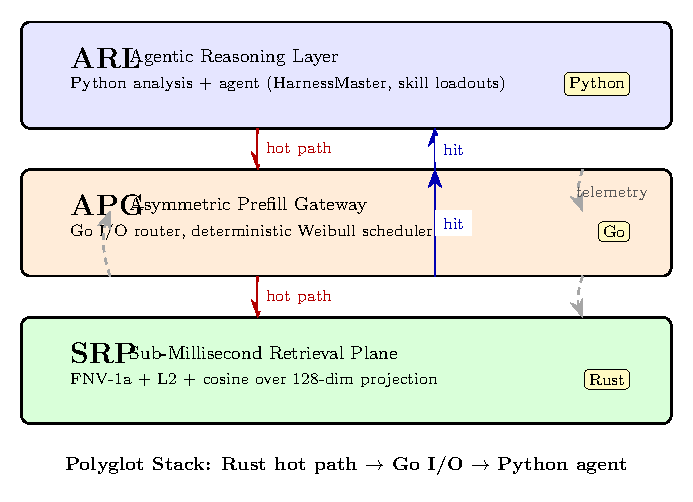
\includegraphics[width=\columnwidth]{figures/fig_polyglot_stack.pdf}
\caption{The polyglot stack at a glance. The four production languages
own four distinct invariants (bitwise determinism, goroutine
isolation, ecosystem breadth, cache-line granularity). The FNV-1a +
$L_2$ + cosine + throughput formulas are the common mathematical
substrate; the polyglot implementation is the engineering
realization.}
\label{fig:polyglot-stack}
\end{figure}

\begin{remark}[Why not a single language?]
A reasonable reviewer question is ``why not implement the entire stack
in Rust?''. The answer is that the SRP, APG, and CCEBH are correctly
implemented in Rust (they all share the bitwise-determinism invariant),
but the ARL is correctly implemented in Python (the ecosystem-breadth
invariant dominates) and the APG is correctly implemented in Go (the
goroutine-isolation invariant dominates). A single-language
implementation would force a compromise on at least one invariant and
would not produce the $25/25$ concurrency-stability result. The
polyglot stack is the \emph{engineering realization} of the
mathematical stack, not a violation of the ``single language'' heuristic.
\end{remark}

